\documentclass[1p]{elsarticle_modified}
%\bibliographystyle{elsarticle-num}

%\usepackage[colorlinks]{hyperref}
%\usepackage{abbrmath_seonhwa} %\Abb, \Ascr, \Acal ,\Abf, \Afrak
\usepackage{amsfonts}
\usepackage{amssymb}
\usepackage{amsmath}
\usepackage{amsthm}
\usepackage{scalefnt}
\usepackage{amsbsy}
\usepackage{kotex}
\usepackage{caption}
\usepackage{subfig}
\usepackage{color}
\usepackage{graphicx}
\usepackage{xcolor} %% white, black, red, green, blue, cyan, magenta, yellow
\usepackage{float}
\usepackage{setspace}
\usepackage{hyperref}

\usepackage{tikz}
\usetikzlibrary{arrows}

\usepackage{multirow}
\usepackage{array} % fixed length table
\usepackage{hhline}

%%%%%%%%%%%%%%%%%%%%%
\makeatletter
\renewcommand*\env@matrix[1][\arraystretch]{%
	\edef\arraystretch{#1}%
	\hskip -\arraycolsep
	\let\@ifnextchar\new@ifnextchar
	\array{*\c@MaxMatrixCols c}}
\makeatother %https://tex.stackexchange.com/questions/14071/how-can-i-increase-the-line-spacing-in-a-matrix
%%%%%%%%%%%%%%%

\usepackage[normalem]{ulem}

\newcommand{\msout}[1]{\ifmmode\text{\sout{\ensuremath{#1}}}\else\sout{#1}\fi}
%SOURCE: \msout is \stkout macro in https://tex.stackexchange.com/questions/20609/strikeout-in-math-mode

\newcommand{\cancel}[1]{
	\ifmmode
	{\color{red}\msout{#1}}
	\else
	{\color{red}\sout{#1}}
	\fi
}

\newcommand{\add}[1]{
	{\color{blue}\uwave{#1}}
}

\newcommand{\replace}[2]{
	\ifmmode
	{\color{red}\msout{#1}}{\color{blue}\uwave{#2}}
	\else
	{\color{red}\sout{#1}}{\color{blue}\uwave{#2}}
	\fi
}

\newcommand{\Sol}{\mathcal{S}} %segment
\newcommand{\D}{D} %diagram
\newcommand{\A}{\mathcal{A}} %arc


%%%%%%%%%%%%%%%%%%%%%%%%%%%%%5 test

\def\sl{\operatorname{\textup{SL}}(2,\Cbb)}
\def\psl{\operatorname{\textup{PSL}}(2,\Cbb)}
\def\quan{\mkern 1mu \triangleright \mkern 1mu}

\theoremstyle{definition}
\newtheorem{thm}{Theorem}[section]
\newtheorem{prop}[thm]{Proposition}
\newtheorem{lem}[thm]{Lemma}
\newtheorem{ques}[thm]{Question}
\newtheorem{cor}[thm]{Corollary}
\newtheorem{defn}[thm]{Definition}
\newtheorem{exam}[thm]{Example}
\newtheorem{rmk}[thm]{Remark}
\newtheorem{alg}[thm]{Algorithm}

\newcommand{\I}{\sqrt{-1}}
\begin{document}

%\begin{frontmatter}
%
%\title{Boundary parabolic representations of knots up to 8 crossings}
%
%%% Group authors per affiliation:
%\author{Yunhi Cho} 
%\address{Department of Mathematics, University of Seoul, Seoul, Korea}
%\ead{yhcho@uos.ac.kr}
%
%
%\author{Seonhwa Kim} %\fnref{s_kim}}
%\address{Center for Geometry and Physics, Institute for Basic Science, Pohang, 37673, Korea}
%\ead{ryeona17@ibs.re.kr}
%
%\author{Hyuk Kim}
%\address{Department of Mathematical Sciences, Seoul National University, Seoul 08826, Korea}
%\ead{hyukkim@snu.ac.kr}
%
%\author{Seokbeom Yoon}
%\address{Department of Mathematical Sciences, Seoul National University, Seoul, 08826,  Korea}
%\ead{sbyoon15@snu.ac.kr}
%
%\begin{abstract}
%We find all boundary parabolic representation of knots up to 8 crossings.
%
%\end{abstract}
%\begin{keyword}
%    \MSC[2010] 57M25 
%\end{keyword}
%
%\end{frontmatter}

%\linenumbers
%\tableofcontents
%
\newcommand\colored[1]{\textcolor{white}{\rule[-0.35ex]{0.8em}{1.4ex}}\kern-0.8em\color{red} #1}%
%\newcommand\colored[1]{\textcolor{white}{ #1}\kern-2.17ex	\textcolor{white}{ #1}\kern-1.81ex	\textcolor{white}{ #1}\kern-2.15ex\color{red}#1	}

{\Large $\underline{12n_{0237}~(K12n_{0237})}$}

\setlength{\tabcolsep}{10pt}
\renewcommand{\arraystretch}{1.6}
\vspace{1cm}\begin{tabular}{m{100pt}>{\centering\arraybackslash}m{274pt}}
\multirow{5}{120pt}{
	\centering
	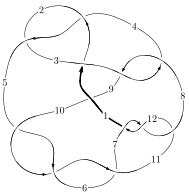
\includegraphics[width=112pt]{../../../GIT/diagram.site/Diagrams/png/2326_12n_0237.png}\\
\ \ \ A knot diagram\footnotemark}&
\allowdisplaybreaks
\textbf{Linearized knot diagam} \\
\cline{2-2}
 &
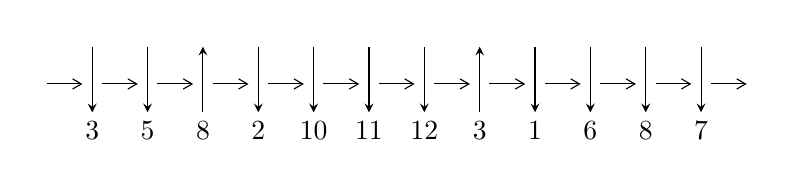
\begin{tikzpicture}[x=20pt, y=17pt]
	% nodes
	\node (C0) at (0, 0) {};
	\node (C1) at (1, 0) {};
	\node (C1U) at (1, +1) {};
	\node (C1D) at (1, -1) {3};

	\node (C2) at (2, 0) {};
	\node (C2U) at (2, +1) {};
	\node (C2D) at (2, -1) {5};

	\node (C3) at (3, 0) {};
	\node (C3U) at (3, +1) {};
	\node (C3D) at (3, -1) {8};

	\node (C4) at (4, 0) {};
	\node (C4U) at (4, +1) {};
	\node (C4D) at (4, -1) {2};

	\node (C5) at (5, 0) {};
	\node (C5U) at (5, +1) {};
	\node (C5D) at (5, -1) {10};

	\node (C6) at (6, 0) {};
	\node (C6U) at (6, +1) {};
	\node (C6D) at (6, -1) {11};

	\node (C7) at (7, 0) {};
	\node (C7U) at (7, +1) {};
	\node (C7D) at (7, -1) {12};

	\node (C8) at (8, 0) {};
	\node (C8U) at (8, +1) {};
	\node (C8D) at (8, -1) {3};

	\node (C9) at (9, 0) {};
	\node (C9U) at (9, +1) {};
	\node (C9D) at (9, -1) {1};

	\node (C10) at (10, 0) {};
	\node (C10U) at (10, +1) {};
	\node (C10D) at (10, -1) {6};

	\node (C11) at (11, 0) {};
	\node (C11U) at (11, +1) {};
	\node (C11D) at (11, -1) {8};

	\node (C12) at (12, 0) {};
	\node (C12U) at (12, +1) {};
	\node (C12D) at (12, -1) {7};
	\node (C13) at (13, 0) {};

	% arrows
	\draw[->,>={angle 60}]
	(C0) edge (C1) (C1) edge (C2) (C2) edge (C3) (C3) edge (C4) (C4) edge (C5) (C5) edge (C6) (C6) edge (C7) (C7) edge (C8) (C8) edge (C9) (C9) edge (C10) (C10) edge (C11) (C11) edge (C12) (C12) edge (C13) ;	\draw[->,>=stealth]
	(C1U) edge (C1D) (C2U) edge (C2D) (C3D) edge (C3U) (C4U) edge (C4D) (C5U) edge (C5D) (C6U) edge (C6D) (C7U) edge (C7D) (C8D) edge (C8U) (C9U) edge (C9D) (C10U) edge (C10D) (C11U) edge (C11D) (C12U) edge (C12D) ;
	\end{tikzpicture} \\
\hhline{~~} \\& 
\textbf{Solving Sequence} \\ \cline{2-2} 
 &
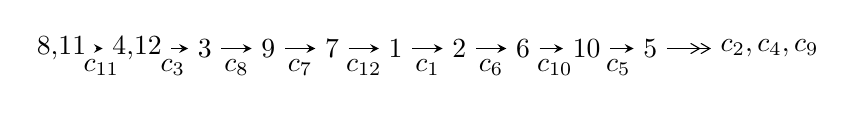
\begin{tikzpicture}[x=23pt, y=7pt]
	% node
	\node (A0) at (-1/8, 0) {8,11};
	\node (A1) at (17/16, 0) {4,12};
	\node (A2) at (17/8, 0) {3};
	\node (A3) at (25/8, 0) {9};
	\node (A4) at (33/8, 0) {7};
	\node (A5) at (41/8, 0) {1};
	\node (A6) at (49/8, 0) {2};
	\node (A7) at (57/8, 0) {6};
	\node (A8) at (65/8, 0) {10};
	\node (A9) at (73/8, 0) {5};
	\node (C1) at (1/2, -1) {$c_{11}$};
	\node (C2) at (13/8, -1) {$c_{3}$};
	\node (C3) at (21/8, -1) {$c_{8}$};
	\node (C4) at (29/8, -1) {$c_{7}$};
	\node (C5) at (37/8, -1) {$c_{12}$};
	\node (C6) at (45/8, -1) {$c_{1}$};
	\node (C7) at (53/8, -1) {$c_{6}$};
	\node (C8) at (61/8, -1) {$c_{10}$};
	\node (C9) at (69/8, -1) {$c_{5}$};
	\node (A10) at (11, 0) {$c_{2},c_{4},c_{9}$};

	% edge
	\draw[->,>=stealth]	
	(A0) edge (A1) (A1) edge (A2) (A2) edge (A3) (A3) edge (A4) (A4) edge (A5) (A5) edge (A6) (A6) edge (A7) (A7) edge (A8) (A8) edge (A9) ;
	\draw[->>,>={angle 60}]	
	(A9) edge (A10);
\end{tikzpicture} \\ 

\end{tabular} \\

\footnotetext{
The image of knot diagram is generated by the software ``\textbf{Draw programme}" developed by Andrew Bartholomew(\url{http://www.layer8.co.uk/maths/draw/index.htm\#Running-draw}), where we modified some parts for our purpose(\url{https://github.com/CATsTAILs/LinksPainter}).
}\phantom \\ \newline 
\centering \textbf{Ideals for irreducible components\footnotemark of $X_{\text{par}}$} 
 
\begin{align*}
I^u_{1}&=\langle 
u^{41}+u^{40}+\cdots+b+2 u,\;u^{41}+u^{40}+\cdots+a-4 u,\;u^{42}+2 u^{41}+\cdots+u+1\rangle \\
I^u_{2}&=\langle 
- u^4+u^3-2 u^2+b+u,\;a,\;u^6- u^5+3 u^4-2 u^3+2 u^2- u-1\rangle \\
\\
\end{align*}
\raggedright * 2 irreducible components of $\dim_{\mathbb{C}}=0$, with total 48 representations.\\
\footnotetext{All coefficients of polynomials are rational numbers. But the coefficients are sometimes approximated in decimal forms when there is not enough margin.}
\newpage
\renewcommand{\arraystretch}{1}
\centering \section*{I. $I^u_{1}= \langle u^{41}+u^{40}+\cdots+b+2 u,\;u^{41}+u^{40}+\cdots+a-4 u,\;u^{42}+2 u^{41}+\cdots+u+1 \rangle$}
\flushleft \textbf{(i) Arc colorings}\\
\begin{tabular}{m{7pt} m{180pt} m{7pt} m{180pt} }
\flushright $a_{8}=$&$\begin{pmatrix}0\\u\end{pmatrix}$ \\
\flushright $a_{11}=$&$\begin{pmatrix}1\\0\end{pmatrix}$ \\
\flushright $a_{4}=$&$\begin{pmatrix}- u^{41}- u^{40}+\cdots+2 u^2+4 u\\- u^{41}- u^{40}+\cdots-8 u^2-2 u\end{pmatrix}$ \\
\flushright $a_{12}=$&$\begin{pmatrix}1\\u^2\end{pmatrix}$ \\
\flushright $a_{3}=$&$\begin{pmatrix}- u^{41}- u^{40}+\cdots+2 u^2+4 u\\- u^{41}-2 u^{40}+\cdots-2 u-1\end{pmatrix}$ \\
\flushright $a_{9}=$&$\begin{pmatrix}u^{12}+5 u^{10}+9 u^8+4 u^6-6 u^4-5 u^2+1\\u^{14}+6 u^{12}+13 u^{10}+10 u^8-4 u^6-8 u^4- u^2\end{pmatrix}$ \\
\flushright $a_{7}=$&$\begin{pmatrix}u\\u^3+u\end{pmatrix}$ \\
\flushright $a_{1}=$&$\begin{pmatrix}u^2+1\\u^4+2 u^2\end{pmatrix}$ \\
\flushright $a_{2}=$&$\begin{pmatrix}u^9+4 u^7+5 u^5-3 u\\- u^{37}- u^{36}+\cdots+8 u^2+2 u\end{pmatrix}$ \\
\flushright $a_{6}=$&$\begin{pmatrix}u^3+2 u\\u^3+u\end{pmatrix}$ \\
\flushright $a_{10}=$&$\begin{pmatrix}- u^6-3 u^4-2 u^2+1\\- u^6-2 u^4- u^2\end{pmatrix}$ \\
\flushright $a_{5}=$&$\begin{pmatrix}- u^9-4 u^7-5 u^5+3 u\\- u^9-3 u^7-3 u^5+u\end{pmatrix}$\\&\end{tabular}
\flushleft \textbf{(ii) Obstruction class $= -1$}\\~\\
\flushleft \textbf{(iii) Cusp Shapes $= -4 u^{41}-8 u^{40}+\cdots+15 u-9$}\\~\\
\newpage\renewcommand{\arraystretch}{1}
\flushleft \textbf{(iv) u-Polynomials at the component}\newline \\
\begin{tabular}{m{50pt}|m{274pt}}
Crossings & \hspace{64pt}u-Polynomials at each crossing \\
\hline $$\begin{aligned}c_{1}\end{aligned}$$&$\begin{aligned}
&u^{42}+13 u^{41}+\cdots+28 u+1
\end{aligned}$\\
\hline $$\begin{aligned}c_{2},c_{4}\end{aligned}$$&$\begin{aligned}
&u^{42}-7 u^{41}+\cdots-8 u+1
\end{aligned}$\\
\hline $$\begin{aligned}c_{3},c_{8}\end{aligned}$$&$\begin{aligned}
&u^{42}+u^{41}+\cdots+192 u+64
\end{aligned}$\\
\hline $$\begin{aligned}c_{5},c_{6},c_{10}\end{aligned}$$&$\begin{aligned}
&u^{42}-2 u^{41}+\cdots-55 u+17
\end{aligned}$\\
\hline $$\begin{aligned}c_{7},c_{11},c_{12}\end{aligned}$$&$\begin{aligned}
&u^{42}+2 u^{41}+\cdots+u+1
\end{aligned}$\\
\hline $$\begin{aligned}c_{9}\end{aligned}$$&$\begin{aligned}
&u^{42}+2 u^{41}+\cdots+5 u+1
\end{aligned}$\\
\hline
\end{tabular}\\~\\
\newpage\renewcommand{\arraystretch}{1}
\flushleft \textbf{(v) Riley Polynomials at the component}\newline \\
\begin{tabular}{m{50pt}|m{274pt}}
Crossings & \hspace{64pt}Riley Polynomials at each crossing \\
\hline $$\begin{aligned}c_{1}\end{aligned}$$&$\begin{aligned}
&y^{42}+39 y^{41}+\cdots-212 y+1
\end{aligned}$\\
\hline $$\begin{aligned}c_{2},c_{4}\end{aligned}$$&$\begin{aligned}
&y^{42}-13 y^{41}+\cdots-28 y+1
\end{aligned}$\\
\hline $$\begin{aligned}c_{3},c_{8}\end{aligned}$$&$\begin{aligned}
&y^{42}-39 y^{41}+\cdots-90112 y+4096
\end{aligned}$\\
\hline $$\begin{aligned}c_{5},c_{6},c_{10}\end{aligned}$$&$\begin{aligned}
&y^{42}-38 y^{41}+\cdots-4011 y+289
\end{aligned}$\\
\hline $$\begin{aligned}c_{7},c_{11},c_{12}\end{aligned}$$&$\begin{aligned}
&y^{42}+34 y^{41}+\cdots-19 y+1
\end{aligned}$\\
\hline $$\begin{aligned}c_{9}\end{aligned}$$&$\begin{aligned}
&y^{42}+46 y^{41}+\cdots-19 y+1
\end{aligned}$\\
\hline
\end{tabular}\\~\\
\newpage\flushleft \textbf{(vi) Complex Volumes and Cusp Shapes}
$$\begin{array}{c|c|c}  
\text{Solutions to }I^u_{1}& \I (\text{vol} + \sqrt{-1}CS) & \text{Cusp shape}\\
 \hline 
\begin{aligned}
u &= \phantom{-}0.884997\phantom{ +0.000000I} \\
a &= -0.685840\phantom{ +0.000000I} \\
b &= -0.554744\phantom{ +0.000000I}\end{aligned}
 & -8.59934\phantom{ +0.000000I} & -6.83080\phantom{ +0.000000I} \\ \hline\begin{aligned}
u &= -0.860411 + 0.091340 I \\
a &= \phantom{-}1.60817 + 0.83486 I \\
b &= \phantom{-}0.281208 + 1.248210 I\end{aligned}
 & -1.28738 + 8.63776 I & -11.30852 - 5.50570 I \\ \hline\begin{aligned}
u &= -0.860411 - 0.091340 I \\
a &= \phantom{-}1.60817 - 0.83486 I \\
b &= \phantom{-}0.281208 - 1.248210 I\end{aligned}
 & -1.28738 - 8.63776 I & -11.30852 + 5.50570 I \\ \hline\begin{aligned}
u &= -0.819362 + 0.102352 I \\
a &= -1.76027 - 0.48960 I \\
b &= -0.358516 - 0.802687 I\end{aligned}
 & \phantom{-}0.15821 + 2.18866 I & -9.63326 - 1.25581 I \\ \hline\begin{aligned}
u &= -0.819362 - 0.102352 I \\
a &= -1.76027 + 0.48960 I \\
b &= -0.358516 + 0.802687 I\end{aligned}
 & \phantom{-}0.15821 - 2.18866 I & -9.63326 + 1.25581 I \\ \hline\begin{aligned}
u &= -0.818580\phantom{ +0.000000I} \\
a &= \phantom{-}1.24094\phantom{ +0.000000I} \\
b &= -0.564691\phantom{ +0.000000I}\end{aligned}
 & -7.20526\phantom{ +0.000000I} & -12.4480\phantom{ +0.000000I} \\ \hline\begin{aligned}
u &= \phantom{-}0.813444 + 0.036008 I \\
a &= -0.240335 - 1.364030 I \\
b &= -0.236106 - 1.145350 I\end{aligned}
 & -5.56172 - 2.39562 I & -13.13795 + 3.14651 I \\ \hline\begin{aligned}
u &= \phantom{-}0.813444 - 0.036008 I \\
a &= -0.240335 + 1.364030 I \\
b &= -0.236106 + 1.145350 I\end{aligned}
 & -5.56172 + 2.39562 I & -13.13795 - 3.14651 I \\ \hline\begin{aligned}
u &= -0.360418 + 1.144850 I \\
a &= \phantom{-}0.461015 + 1.052370 I \\
b &= \phantom{-}0.396025 + 0.874829 I\end{aligned}
 & \phantom{-}3.34850 + 2.08589 I & -6.37713 - 2.84313 I \\ \hline\begin{aligned}
u &= -0.360418 - 1.144850 I \\
a &= \phantom{-}0.461015 - 1.052370 I \\
b &= \phantom{-}0.396025 - 0.874829 I\end{aligned}
 & \phantom{-}3.34850 - 2.08589 I & -6.37713 + 2.84313 I\\
 \hline 
 \end{array}$$\newpage$$\begin{array}{c|c|c}  
\text{Solutions to }I^u_{1}& \I (\text{vol} + \sqrt{-1}CS) & \text{Cusp shape}\\
 \hline 
\begin{aligned}
u &= \phantom{-}0.039780 + 1.228480 I \\
a &= -0.408011 + 0.443145 I \\
b &= \phantom{-}0.69289 + 2.43964 I\end{aligned}
 & \phantom{-}1.48060 - 0.96666 I & -6.26750 - 1.40491 I \\ \hline\begin{aligned}
u &= \phantom{-}0.039780 - 1.228480 I \\
a &= -0.408011 - 0.443145 I \\
b &= \phantom{-}0.69289 - 2.43964 I\end{aligned}
 & \phantom{-}1.48060 + 0.96666 I & -6.26750 + 1.40491 I \\ \hline\begin{aligned}
u &= -0.193377 + 1.231330 I \\
a &= \phantom{-}0.262816 + 0.483914 I \\
b &= \phantom{-}0.802069 + 0.546478 I\end{aligned}
 & \phantom{-}2.73948 + 2.47038 I & -3.06420 - 3.92417 I \\ \hline\begin{aligned}
u &= -0.193377 - 1.231330 I \\
a &= \phantom{-}0.262816 - 0.483914 I \\
b &= \phantom{-}0.802069 - 0.546478 I\end{aligned}
 & \phantom{-}2.73948 - 2.47038 I & -3.06420 + 3.92417 I \\ \hline\begin{aligned}
u &= -0.415470 + 1.179020 I \\
a &= -0.775903 - 0.927476 I \\
b &= -0.095078 - 0.588213 I\end{aligned}
 & \phantom{-}2.05152 - 4.06193 I & -8.19749 + 0. I\phantom{ +0.000000I} \\ \hline\begin{aligned}
u &= -0.415470 - 1.179020 I \\
a &= -0.775903 + 0.927476 I \\
b &= -0.095078 + 0.588213 I\end{aligned}
 & \phantom{-}2.05152 + 4.06193 I & -8.19749 + 0. I\phantom{ +0.000000I} \\ \hline\begin{aligned}
u &= \phantom{-}0.357741 + 1.238750 I \\
a &= -0.744213 - 0.408723 I \\
b &= \phantom{-}0.418778 - 1.322100 I\end{aligned}
 & -1.85166 - 1.82090 I & -9.63780 + 0. I\phantom{ +0.000000I} \\ \hline\begin{aligned}
u &= \phantom{-}0.357741 - 1.238750 I \\
a &= -0.744213 + 0.408723 I \\
b &= \phantom{-}0.418778 + 1.322100 I\end{aligned}
 & -1.85166 + 1.82090 I & -9.63780 + 0. I\phantom{ +0.000000I} \\ \hline\begin{aligned}
u &= -0.079247 + 1.295310 I \\
a &= \phantom{-}0.637223 - 0.258877 I \\
b &= \phantom{-}1.01766 - 1.34640 I\end{aligned}
 & \phantom{-}4.02758 + 2.15699 I & \phantom{-0.000000 } 0 \\ \hline\begin{aligned}
u &= -0.079247 - 1.295310 I \\
a &= \phantom{-}0.637223 + 0.258877 I \\
b &= \phantom{-}1.01766 + 1.34640 I\end{aligned}
 & \phantom{-}4.02758 - 2.15699 I & \phantom{-0.000000 } 0\\
 \hline 
 \end{array}$$\newpage$$\begin{array}{c|c|c}  
\text{Solutions to }I^u_{1}& \I (\text{vol} + \sqrt{-1}CS) & \text{Cusp shape}\\
 \hline 
\begin{aligned}
u &= -0.365234 + 1.269190 I \\
a &= -0.284658 - 0.718402 I \\
b &= -0.34989 - 2.35592 I\end{aligned}
 & -3.26541 + 4.25757 I & \phantom{-0.000000 } 0 \\ \hline\begin{aligned}
u &= -0.365234 - 1.269190 I \\
a &= -0.284658 + 0.718402 I \\
b &= -0.34989 + 2.35592 I\end{aligned}
 & -3.26541 - 4.25757 I & \phantom{-0.000000 } 0 \\ \hline\begin{aligned}
u &= \phantom{-}0.517463 + 0.417209 I \\
a &= \phantom{-}1.47848 - 1.77950 I \\
b &= \phantom{-}0.187293 - 1.152780 I\end{aligned}
 & \phantom{-}4.73868 - 4.97358 I & -7.62188 + 6.30595 I \\ \hline\begin{aligned}
u &= \phantom{-}0.517463 - 0.417209 I \\
a &= \phantom{-}1.47848 + 1.77950 I \\
b &= \phantom{-}0.187293 + 1.152780 I\end{aligned}
 & \phantom{-}4.73868 + 4.97358 I & -7.62188 - 6.30595 I \\ \hline\begin{aligned}
u &= \phantom{-}0.443990 + 0.494284 I \\
a &= -1.67760 + 1.53589 I \\
b &= -0.210344 + 0.860490 I\end{aligned}
 & \phantom{-}5.02884 + 1.46246 I & -6.53686 + 0.89586 I \\ \hline\begin{aligned}
u &= \phantom{-}0.443990 - 0.494284 I \\
a &= -1.67760 - 1.53589 I \\
b &= -0.210344 - 0.860490 I\end{aligned}
 & \phantom{-}5.02884 - 1.46246 I & -6.53686 - 0.89586 I \\ \hline\begin{aligned}
u &= \phantom{-}0.418536 + 1.277910 I \\
a &= \phantom{-}0.134196 - 0.433061 I \\
b &= \phantom{-}0.636951 - 0.103857 I\end{aligned}
 & -4.63050 - 4.66445 I & \phantom{-0.000000 } 0 \\ \hline\begin{aligned}
u &= \phantom{-}0.418536 - 1.277910 I \\
a &= \phantom{-}0.134196 + 0.433061 I \\
b &= \phantom{-}0.636951 + 0.103857 I\end{aligned}
 & -4.63050 + 4.66445 I & \phantom{-0.000000 } 0 \\ \hline\begin{aligned}
u &= \phantom{-}0.361948 + 1.295330 I \\
a &= \phantom{-}0.843712 + 0.183840 I \\
b &= \phantom{-}0.34096 + 1.49506 I\end{aligned}
 & -1.40855 - 6.62685 I & \phantom{-0.000000 } 0 \\ \hline\begin{aligned}
u &= \phantom{-}0.361948 - 1.295330 I \\
a &= \phantom{-}0.843712 - 0.183840 I \\
b &= \phantom{-}0.34096 - 1.49506 I\end{aligned}
 & -1.40855 + 6.62685 I & \phantom{-0.000000 } 0\\
 \hline 
 \end{array}$$\newpage$$\begin{array}{c|c|c}  
\text{Solutions to }I^u_{1}& \I (\text{vol} + \sqrt{-1}CS) & \text{Cusp shape}\\
 \hline 
\begin{aligned}
u &= -0.361210 + 1.333990 I \\
a &= \phantom{-}0.133728 + 1.145250 I \\
b &= \phantom{-}1.68733 + 2.67654 I\end{aligned}
 & \phantom{-}4.66389 + 6.44264 I & \phantom{-0.000000 } 0 \\ \hline\begin{aligned}
u &= -0.361210 - 1.333990 I \\
a &= \phantom{-}0.133728 - 1.145250 I \\
b &= \phantom{-}1.68733 - 2.67654 I\end{aligned}
 & \phantom{-}4.66389 - 6.44264 I & \phantom{-0.000000 } 0 \\ \hline\begin{aligned}
u &= \phantom{-}0.108456 + 1.380140 I \\
a &= \phantom{-}0.156921 - 1.186400 I \\
b &= \phantom{-}1.07791 - 4.11722 I\end{aligned}
 & \phantom{-}10.88470 - 0.27094 I & \phantom{-0.000000 } 0 \\ \hline\begin{aligned}
u &= \phantom{-}0.108456 - 1.380140 I \\
a &= \phantom{-}0.156921 + 1.186400 I \\
b &= \phantom{-}1.07791 + 4.11722 I\end{aligned}
 & \phantom{-}10.88470 + 0.27094 I & \phantom{-0.000000 } 0 \\ \hline\begin{aligned}
u &= \phantom{-}0.146369 + 1.377200 I \\
a &= \phantom{-}0.141022 + 1.192190 I \\
b &= -0.84503 + 4.22749 I\end{aligned}
 & \phantom{-}10.39390 - 7.18776 I & \phantom{-0.000000 } 0 \\ \hline\begin{aligned}
u &= \phantom{-}0.146369 - 1.377200 I \\
a &= \phantom{-}0.141022 - 1.192190 I \\
b &= -0.84503 - 4.22749 I\end{aligned}
 & \phantom{-}10.39390 + 7.18776 I & \phantom{-0.000000 } 0 \\ \hline\begin{aligned}
u &= -0.385158 + 1.335160 I \\
a &= \phantom{-}0.110632 - 1.155620 I \\
b &= -1.67195 - 2.97617 I\end{aligned}
 & \phantom{-}3.18564 + 13.11100 I & \phantom{-0.000000 } 0 \\ \hline\begin{aligned}
u &= -0.385158 - 1.335160 I \\
a &= \phantom{-}0.110632 + 1.155620 I \\
b &= -1.67195 + 2.97617 I\end{aligned}
 & \phantom{-}3.18564 - 13.11100 I & \phantom{-0.000000 } 0 \\ \hline\begin{aligned}
u &= -0.492418\phantom{ +0.000000I} \\
a &= -0.979682\phantom{ +0.000000I} \\
b &= -0.240678\phantom{ +0.000000I}\end{aligned}
 & -0.983238\phantom{ +0.000000I} & -9.79060\phantom{ +0.000000I} \\ \hline\begin{aligned}
u &= -0.283222 + 0.253637 I \\
a &= -1.15749 + 1.43241 I \\
b &= -0.099702 + 0.442777 I\end{aligned}
 & -0.614323 + 0.919516 I & -9.08610 - 7.37537 I\\
 \hline 
 \end{array}$$\newpage$$\begin{array}{c|c|c}  
\text{Solutions to }I^u_{1}& \I (\text{vol} + \sqrt{-1}CS) & \text{Cusp shape}\\
 \hline 
\begin{aligned}
u &= -0.283222 - 0.253637 I \\
a &= -1.15749 - 1.43241 I \\
b &= -0.099702 - 0.442777 I\end{aligned}
 & -0.614323 - 0.919516 I & -9.08610 + 7.37537 I \\ \hline\begin{aligned}
u &= \phantom{-}0.256764\phantom{ +0.000000I} \\
a &= \phantom{-}1.58568\phantom{ +0.000000I} \\
b &= -0.984824\phantom{ +0.000000I}\end{aligned}
 & -2.02811\phantom{ +0.000000I} & \phantom{-}1.75710\phantom{ +0.000000I}\\
 \hline 
 \end{array}$$\newpage\newpage\renewcommand{\arraystretch}{1}
\centering \section*{II. $I^u_{2}= \langle - u^4+u^3-2 u^2+b+u,\;a,\;u^6- u^5+3 u^4-2 u^3+2 u^2- u-1 \rangle$}
\flushleft \textbf{(i) Arc colorings}\\
\begin{tabular}{m{7pt} m{180pt} m{7pt} m{180pt} }
\flushright $a_{8}=$&$\begin{pmatrix}0\\u\end{pmatrix}$ \\
\flushright $a_{11}=$&$\begin{pmatrix}1\\0\end{pmatrix}$ \\
\flushright $a_{4}=$&$\begin{pmatrix}0\\u^4- u^3+2 u^2- u\end{pmatrix}$ \\
\flushright $a_{12}=$&$\begin{pmatrix}1\\u^2\end{pmatrix}$ \\
\flushright $a_{3}=$&$\begin{pmatrix}0\\u^4- u^3+2 u^2- u\end{pmatrix}$ \\
\flushright $a_{9}=$&$\begin{pmatrix}0\\u\end{pmatrix}$ \\
\flushright $a_{7}=$&$\begin{pmatrix}u\\u^3+u\end{pmatrix}$ \\
\flushright $a_{1}=$&$\begin{pmatrix}u^2+1\\u^4+2 u^2\end{pmatrix}$ \\
\flushright $a_{2}=$&$\begin{pmatrix}u^2+1\\2 u^4- u^3+4 u^2- u\end{pmatrix}$ \\
\flushright $a_{6}=$&$\begin{pmatrix}u^3+2 u\\u^3+u\end{pmatrix}$ \\
\flushright $a_{10}=$&$\begin{pmatrix}- u^5-2 u^3- u\\- u^5+u^4-2 u^3+u^2- u-1\end{pmatrix}$ \\
\flushright $a_{5}=$&$\begin{pmatrix}- u^2-1\\- u^4-2 u^2\end{pmatrix}$\\&\end{tabular}
\flushleft \textbf{(ii) Obstruction class $= 1$}\\~\\
\flushleft \textbf{(iii) Cusp Shapes $= -5 u^4+6 u^3-11 u^2+6 u-17$}\\~\\
\newpage\renewcommand{\arraystretch}{1}
\flushleft \textbf{(iv) u-Polynomials at the component}\newline \\
\begin{tabular}{m{50pt}|m{274pt}}
Crossings & \hspace{64pt}u-Polynomials at each crossing \\
\hline $$\begin{aligned}c_{1},c_{2}\end{aligned}$$&$\begin{aligned}
&(u-1)^6
\end{aligned}$\\
\hline $$\begin{aligned}c_{3},c_{8}\end{aligned}$$&$\begin{aligned}
&u^6
\end{aligned}$\\
\hline $$\begin{aligned}c_{4}\end{aligned}$$&$\begin{aligned}
&(u+1)^6
\end{aligned}$\\
\hline $$\begin{aligned}c_{5},c_{6},c_{9}\end{aligned}$$&$\begin{aligned}
&u^6- u^5-3 u^4+2 u^3+2 u^2+u-1
\end{aligned}$\\
\hline $$\begin{aligned}c_{7}\end{aligned}$$&$\begin{aligned}
&u^6+u^5+3 u^4+2 u^3+2 u^2+u-1
\end{aligned}$\\
\hline $$\begin{aligned}c_{10}\end{aligned}$$&$\begin{aligned}
&u^6+u^5-3 u^4-2 u^3+2 u^2- u-1
\end{aligned}$\\
\hline $$\begin{aligned}c_{11},c_{12}\end{aligned}$$&$\begin{aligned}
&u^6- u^5+3 u^4-2 u^3+2 u^2- u-1
\end{aligned}$\\
\hline
\end{tabular}\\~\\
\newpage\renewcommand{\arraystretch}{1}
\flushleft \textbf{(v) Riley Polynomials at the component}\newline \\
\begin{tabular}{m{50pt}|m{274pt}}
Crossings & \hspace{64pt}Riley Polynomials at each crossing \\
\hline $$\begin{aligned}c_{1},c_{2},c_{4}\end{aligned}$$&$\begin{aligned}
&(y-1)^6
\end{aligned}$\\
\hline $$\begin{aligned}c_{3},c_{8}\end{aligned}$$&$\begin{aligned}
&y^6
\end{aligned}$\\
\hline $$\begin{aligned}c_{5},c_{6},c_{9}\\c_{10}\end{aligned}$$&$\begin{aligned}
&y^6-7 y^5+17 y^4-16 y^3+6 y^2-5 y+1
\end{aligned}$\\
\hline $$\begin{aligned}c_{7},c_{11},c_{12}\end{aligned}$$&$\begin{aligned}
&y^6+5 y^5+9 y^4+4 y^3-6 y^2-5 y+1
\end{aligned}$\\
\hline
\end{tabular}\\~\\
\newpage\flushleft \textbf{(vi) Complex Volumes and Cusp Shapes}
$$\begin{array}{c|c|c}  
\text{Solutions to }I^u_{2}& \I (\text{vol} + \sqrt{-1}CS) & \text{Cusp shape}\\
 \hline 
\begin{aligned}
u &= \phantom{-}0.873214\phantom{ +0.000000I} \\
a &= \phantom{-0.000000 } 0 \\
b &= \phantom{-}0.567375\phantom{ +0.000000I}\end{aligned}
 & -9.30502\phantom{ +0.000000I} & -19.0600\phantom{ +0.000000I} \\ \hline\begin{aligned}
u &= -0.138835 + 1.234450 I \\
a &= \phantom{-0.000000 } 0 \\
b &= -1.35607 + 0.92119 I\end{aligned}
 & \phantom{-}1.31531 + 1.97241 I & -8.22189 - 4.83849 I \\ \hline\begin{aligned}
u &= -0.138835 - 1.234450 I \\
a &= \phantom{-0.000000 } 0 \\
b &= -1.35607 - 0.92119 I\end{aligned}
 & \phantom{-}1.31531 - 1.97241 I & -8.22189 + 4.83849 I \\ \hline\begin{aligned}
u &= \phantom{-}0.408802 + 1.276380 I \\
a &= \phantom{-0.000000 } 0 \\
b &= -0.354716 - 0.801205 I\end{aligned}
 & -5.34051 - 4.59213 I & -15.2853 + 2.7994 I \\ \hline\begin{aligned}
u &= \phantom{-}0.408802 - 1.276380 I \\
a &= \phantom{-0.000000 } 0 \\
b &= -0.354716 + 0.801205 I\end{aligned}
 & -5.34051 + 4.59213 I & -15.2853 - 2.7994 I \\ \hline\begin{aligned}
u &= -0.413150\phantom{ +0.000000I} \\
a &= \phantom{-0.000000 } 0 \\
b &= \phantom{-}0.854195\phantom{ +0.000000I}\end{aligned}
 & -2.38379\phantom{ +0.000000I} & -21.9250\phantom{ +0.000000I}\\
 \hline 
 \end{array}$$\newpage
\newpage\renewcommand{\arraystretch}{1}
\centering \section*{ III. u-Polynomials}
\begin{tabular}{m{50pt}|m{274pt}}
Crossings & \hspace{64pt}u-Polynomials at each crossing \\
\hline $$\begin{aligned}c_{1}\end{aligned}$$&$\begin{aligned}
&((u-1)^6)(u^{42}+13 u^{41}+\cdots+28 u+1)
\end{aligned}$\\
\hline $$\begin{aligned}c_{2}\end{aligned}$$&$\begin{aligned}
&((u-1)^6)(u^{42}-7 u^{41}+\cdots-8 u+1)
\end{aligned}$\\
\hline $$\begin{aligned}c_{3},c_{8}\end{aligned}$$&$\begin{aligned}
&u^6(u^{42}+u^{41}+\cdots+192 u+64)
\end{aligned}$\\
\hline $$\begin{aligned}c_{4}\end{aligned}$$&$\begin{aligned}
&((u+1)^6)(u^{42}-7 u^{41}+\cdots-8 u+1)
\end{aligned}$\\
\hline $$\begin{aligned}c_{5},c_{6}\end{aligned}$$&$\begin{aligned}
&(u^6- u^5-3 u^4+2 u^3+2 u^2+u-1)(u^{42}-2 u^{41}+\cdots-55 u+17)
\end{aligned}$\\
\hline $$\begin{aligned}c_{7}\end{aligned}$$&$\begin{aligned}
&(u^6+u^5+3 u^4+2 u^3+2 u^2+u-1)(u^{42}+2 u^{41}+\cdots+u+1)
\end{aligned}$\\
\hline $$\begin{aligned}c_{9}\end{aligned}$$&$\begin{aligned}
&(u^6- u^5-3 u^4+2 u^3+2 u^2+u-1)(u^{42}+2 u^{41}+\cdots+5 u+1)
\end{aligned}$\\
\hline $$\begin{aligned}c_{10}\end{aligned}$$&$\begin{aligned}
&(u^6+u^5-3 u^4-2 u^3+2 u^2- u-1)(u^{42}-2 u^{41}+\cdots-55 u+17)
\end{aligned}$\\
\hline $$\begin{aligned}c_{11},c_{12}\end{aligned}$$&$\begin{aligned}
&(u^6- u^5+3 u^4-2 u^3+2 u^2- u-1)(u^{42}+2 u^{41}+\cdots+u+1)
\end{aligned}$\\
\hline
\end{tabular}\newpage\renewcommand{\arraystretch}{1}
\centering \section*{ IV. Riley Polynomials}
\begin{tabular}{m{50pt}|m{274pt}}
Crossings & \hspace{64pt}Riley Polynomials at each crossing \\
\hline $$\begin{aligned}c_{1}\end{aligned}$$&$\begin{aligned}
&((y-1)^6)(y^{42}+39 y^{41}+\cdots-212 y+1)
\end{aligned}$\\
\hline $$\begin{aligned}c_{2},c_{4}\end{aligned}$$&$\begin{aligned}
&((y-1)^6)(y^{42}-13 y^{41}+\cdots-28 y+1)
\end{aligned}$\\
\hline $$\begin{aligned}c_{3},c_{8}\end{aligned}$$&$\begin{aligned}
&y^6(y^{42}-39 y^{41}+\cdots-90112 y+4096)
\end{aligned}$\\
\hline $$\begin{aligned}c_{5},c_{6},c_{10}\end{aligned}$$&$\begin{aligned}
&(y^6-7 y^5+17 y^4-16 y^3+6 y^2-5 y+1)\\
&\cdot(y^{42}-38 y^{41}+\cdots-4011 y+289)
\end{aligned}$\\
\hline $$\begin{aligned}c_{7},c_{11},c_{12}\end{aligned}$$&$\begin{aligned}
&(y^6+5 y^5+\cdots-5 y+1)(y^{42}+34 y^{41}+\cdots-19 y+1)
\end{aligned}$\\
\hline $$\begin{aligned}c_{9}\end{aligned}$$&$\begin{aligned}
&(y^6-7 y^5+\cdots-5 y+1)(y^{42}+46 y^{41}+\cdots-19 y+1)
\end{aligned}$\\
\hline
\end{tabular}
\vskip 2pc
\end{document}